\documentclass{beamer}
\usepackage{pharmpresentation}

\title{BlurNet: Defense by Filtering the Feature Maps}
\subtitle{Ravi Raju}

\begin{document}
\begin{frame}
	\titlepage
\end{frame}

\begin{frame}
\frametitle{Outline}
\tableofcontents
\end{frame}

\section{Introduction} % (fold)
\begin{frame}
\frametitle{Vulnerabilities in NNs}
\begin{center}
	
\includegraphics[scale=0.4]{clean_class1.png}
\end{center}
\end{frame}

\begin{frame}
\frametitle{Vulnerabilities in NNs}
\begin{center}
	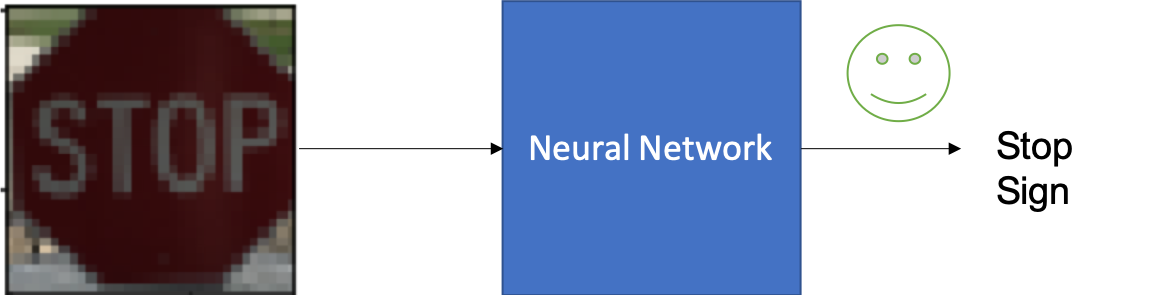
\includegraphics[scale=0.4]{cleanclassification2.png}
\end{center}
\end{frame}


\begin{frame}
\frametitle{Vulnerabilities in NNs cont.}
\begin{center}
	
\includegraphics[scale=0.4]{advclassification1.png}
\end{center}
\end{frame}

\begin{frame}
\frametitle{Vulnerabilities in NNs cont.}
\begin{center}
	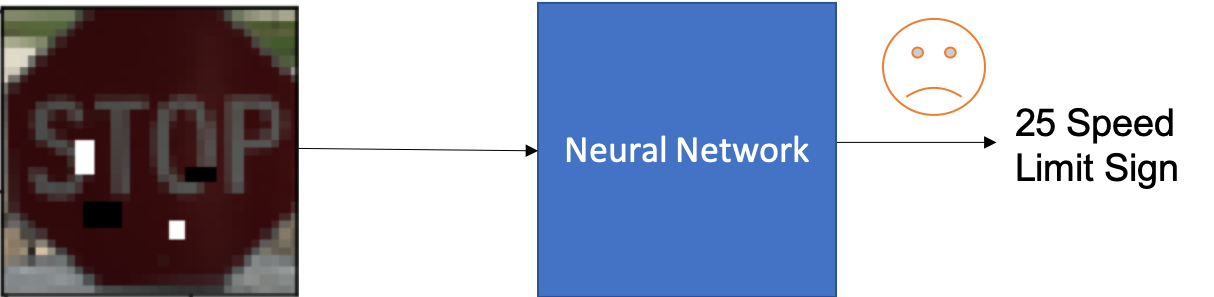
\includegraphics[scale=0.4]{advclassification2.png}
\end{center}
\end{frame}

\begin{frame}
\frametitle{FFT Spectrum of channels}
\begin{center}
	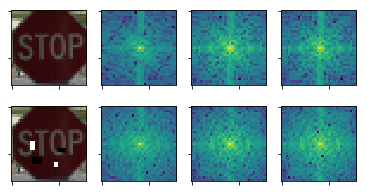
\includegraphics[scale=0.6]{regular_blur.png}
\end{center}
\end{frame}

\begin{frame}
\frametitle{FFT of First Layer}
\begin{center}
	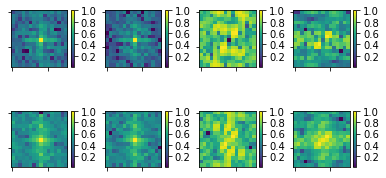
\includegraphics[scale=0.7]{fft_filters.png}
\end{center}
\end{frame}

\begin{frame}
\frametitle{FFT Spectrum of channels}
\begin{center}
	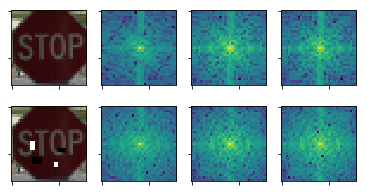
\includegraphics[scale=0.6]{regular_blur.png}
\end{center}
\end{frame}

\begin{frame}
\frametitle{L2 vs Attack Plot}
\begin{center}
	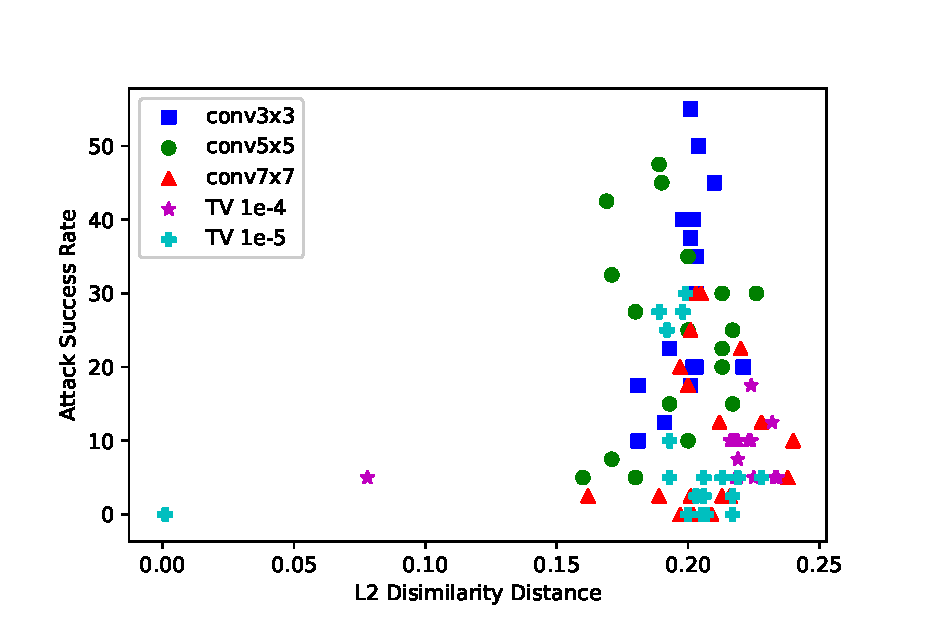
\includegraphics[scale=0.6]{L2vsAttkplot.eps}
\end{center}
\end{frame}

\end{document}